% !TEX spellcheck = en_US
% !TEX encoding = UTF-8

\documentclass[xcolor={x11names, table, dvipsnames}, compress]{beamer}

\usepackage{xcolor}
\usepackage{fontspec}

\usepackage{tikz}
\usepackage{pgfplots}

\usepackage{amsmath, amssymb, amsfonts}
\usepackage{bm}
\usepackage{eso-pic}
\usepackage{graphicx}
\usepackage[hypcap=true]{subcaption}
\usepackage{verbatim}
\usepackage{array}
\usepackage{multirow}
\usepackage{eurosym}
\usepackage{makecell}
\usepackage{hhline}
\usepackage{ifthen}
\usepackage{hyperref}
\usepackage{adjustbox}
% \usepackage[backend=biber]{biblatex}

\pgfplotsset{compat=1.15}
\usetikzlibrary{positioning, shapes, calc, arrows}
\hypersetup{pdfstartview={Fit}}

%% Beamer Layout %%%%%%%%%%%%%%%%%%%%%%%%%%%%%%%%%
\useinnertheme{default}
\usepackage[T1]{fontenc}
\usefonttheme{professionalfonts}

\setbeamerfont{frametitle}{}

\definecolor{BHKpresentationDark}{RGB}{114,133,176}
\definecolor{BHKpresentationDarkGrey}{RGB}{103,116,128}
\definecolor{BHKblue}{RGB}{51,105,153}
\definecolor{BHKLight}{RGB}{239, 249, 255}
\definecolor{BHKDark}{RGB}{0, 134, 202}
\definecolor{BHKRed}{RGB}{173, 0, 53}

\setbeamerfont{title like}{shape=\scshape}
\setbeamercolor*{frametitle}{fg=BHKpresentationDark} 
\setbeamercolor*{lower separation line head}{bg=BHKblue} 
\setbeamercolor*{normal text}{fg=BHKpresentationDarkGrey,bg=white} 
\setbeamercolor*{alerted text}{fg=BHKblue} 
\setbeamercolor*{example text}{fg=black} 
\setbeamercolor*{item}{fg=BHKpresentationDark,bg=gray} 
\setbeamercolor{enumerate item}{fg=BHKpresentationDark}
\setbeamercolor*{structure}{fg=black} 
\setbeamercolor*{palette tertiary}{fg=black,bg=black!10} 
\setbeamercolor*{palette quaternary}{fg=black,bg=black!10} 
\setbeamercovered{transparent}

\setbeamercolor{block body alerted}{bg=BHKLight}
\setbeamercolor{block body}{bg=BHKLight}
\setbeamercolor{block body example}{bg=normal text.bg!90!black}
\setbeamercolor{block title alerted}{use={normal text,alerted text},fg=BHKLight,bg=BHKRed}
\setbeamercolor{block title}{bg=BHKDark, fg=BHKLight}
\setbeamercolor{block title example}{use={normal text,example text},fg=example text.fg!75!normal text.fg,bg=normal text.bg!75!black}

\setbeamertemplate{navigation symbols}{}
\setbeamertemplate{footline}{%
    \begin{beamercolorbox}[wd=\paperwidth]{footlinecolor}
        
\includegraphics[width=\textwidth]{images_presentation/bar_footline.pdf}
    \end{beamercolorbox}%
}

\setbeamertemplate{frametitle}[default][center]
\setbeamertemplate{caption}[numbered]
\setbeamertemplate{section in toc}[sections numbered]
\setbeamertemplate{subsection in toc}[subsections numbered]
\setbeamertemplate{blocks}[rounded][shadow=true]    

\newcolumntype{P}[1]{>{\raggedright\arraybackslash}p{#1}}

\newcommand{\insertsec}{\thesection.~\insertsection}
\newcommand{\insertsubsec}{\thesection.\thesubsection~\insertsubsection}

\AtBeginSection[]{
\begin{frame}
\vfill
\centering
\begin{beamercolorbox}[sep=8pt,center,shadow=true,rounded=true]{title}
    \usebeamerfont{title}\insertsec\par%
\end{beamercolorbox}
\vfill
\end{frame}
}


%%%%%%%%%%%%%%%%%%%%%%%%%%%%%%%%%%%
%% Start of document %%%%%%%%%%%%%%
%%%%%%%%%%%%%%%%%%%%%%%%%%%%%%%%%%%

\begin{document}
%%%% title slide %%%%%%
{
    \setbeamertemplate{footline}{} 
    \begin{frame}
        \begin{flushright}
            \hfill
\includegraphics[width=0.3\textwidth]{images_presentation/logo}
        \end{flushright}
        \begin{flushleft}
            \begin{flushleft}
                \huge \color{BHKpresentationDark} 
                Unlock the potential of medical imaging using deep learning 
            \end{flushleft}

            \hspace{-1cm}
\includegraphics[width=0.8\textwidth]{images_presentation/title_line}\hfill
            
            \date{$~~$}
            \vspace{-1cm}
            {\begin{flushleft}\vspace{-1cm} Joan Marcè i Igual\end{flushleft}}
            \titlepage
        \end{flushleft}
        
        \begin{flushright}
            \vspace{-3cm}
            
\includegraphics[width=.35\textwidth]{images_presentation/pmcp-logo} 

            \vspace{0.5cm}
            
\includegraphics[width=.35\textwidth]{images_presentation/upc-logo} \hspace{1cm}
            
\includegraphics[width=.35\textwidth]{images_presentation/uoft-logo}
        \end{flushright}
    \end{frame}
}

\begin{frame}[allowframebreaks]{Table of Contents}
\tableofcontents
\end{frame}

% !TEX root = ../main.tex

\section{Context}
\begin{frame}{\insertsec}
  \begin{itemize}
    \item Work based on predicting Princess Margaret Cancer Center Dataset's patients survival
    \item Nowadays Machine Learning is widely used
    \item Medical images can be obtained using MRI, PET or CT scans but are underused
    \item Different methods have appeared to analyze these data for image classification,
    object detection, segmentation... usually using deep learning.
    \item Hand-crafted radiomic features can be extracted from medical images
  \end{itemize}
\end{frame}

\subsection{Survival Analysis}
\begin{frame}{\insertsubsec}
  Survival analysis models usually have:
  \begin{itemize}
    \item Baseline data \( x \)
    \item Event \( E \in \{0, 1\} \)
    \item Time \( T \)
    \item Censoring
  \end{itemize}
  
  \begin{block}{Survival function}
    \[
      S(t) = \Pr(T \ge t)
    \]
  \end{block}

  \begin{block}{Hazard function}
  \[
    \lambda(t) = \lim_{\Delta t \rightarrow 0}
    \frac{\Pr(t \le T < t + \Delta t | T \ge t)}{\Delta t}
  \]
  \end{block}

  \begin{block}{Cox Proportional Hazards model}
    \[
      \lambda(t | \bm{x}) = \exp(\bm{x}\bm{\beta}) \cdot \lambda_0 (t)
    \]
  \end{block}
\end{frame}

\begin{frame}

  Casting the survival problem as a ranking is a way of dealing with censored data.
  Conditions:
  \begin{itemize}
    \item Both of them are uncensored (\( \bm{E}_i = \bm{E}_j = 1\))
    \item The uncensored time of one is smaller than the censored survival time of the other
    (\( \bm{T}_i < \bm{T}_j | \bm{E}_i = 1; \bm{E}_j = 0 \))
  \end{itemize}

  \begin{columns}
    \begin{column}{.5\textwidth}
      \begin{figure}
        \centering
        \scalebox{.8}{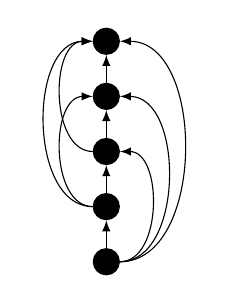
\begin{tikzpicture}[scale=.7]
  \tikzstyle{bDot}=[circle, fill=black, draw]
  \foreach \y in {1,...,5} {
    \node[bDot] (D-\y) at (0, \y) {};
  }

  \foreach \y in {1,...,4} {
    \pgfmathsetmacro{\z}{int(\y + 1)}
    \draw[-latex] (D-\y) -- ({D-\z}.south);
  }

  \foreach \y in {1,...,3} {
    \pgfmathsetmacro{\z}{int(\y + 2)}
    \foreach \j in {\z,...,5} {
      \ifthenelse{\y=2 \OR \y=3}{
        \draw[-latex] (D-\y) to[bend left=90] (D-\j);
      }{
        \draw[-latex] (D-\y) to[bend right=90] (D-\j);
      }
    }
  }
\end{tikzpicture}
}
        \caption{Uncensored data}
      \end{figure}
    \end{column}
    \begin{column}{.5\textwidth}
      \begin{figure}
        \centering
        \scalebox{.8}{\begin{tikzpicture}
  \foreach \y in {1,...,5} {
    \ifthenelse{\y=2 \OR \y=4}{
      \node [circle, fill=white, draw=black] (D-\y) at (0, \y) {};
    }{
      \node [circle, fill=black, draw=black] (D-\y) at (0, \y) {};
    }

    \foreach \y in {3,4,5} {
      \draw [-latex] (D-1) to[bend right=90] (D-\y);
    }

    \foreach \y/\z in {1/2, 3/4} {
      \draw [-latex] (D-\y) -- (D-\z);
    }
    \draw [-latex] (D-3) to[bend left=90] (D-5);
  }
\end{tikzpicture}
}
        \caption{Censored data}
      \end{figure}
    \end{column}
  \end{columns}
\end{frame}

\begin{frame}
  \begin{block}{Good prediction}
    \[
      T_i > T_j \land \hat{T}_i > \hat{T}_j
    \]
  \end{block}

  \begin{block}{Bad prediction}
    \[
      T_i > T_j \land \hat{T}_i < \hat{T}_j
    \]
  \end{block}

  \begin{block}{Concordance Index}
    \[
      CI = \frac{\text{Good predictions}}{\text{Total predictions}} \in [0, 1]
    \]
  \end{block}
\end{frame}

\subsection{Dataset}
\begin{frame}{\insertsubsec}
  \begin{itemize}
    \item Dataset with 671 patients diagnosed of Oropharyngeal Squamous Cell Carcinoma
    \item CT scan of \( 512 \times 512 \) with 100-200 slices
    \item Tumour annotated in provided mask
    \item Clinical information compressed of:
    \begin{itemize}
      \item Subject characteristics
      \item Tumour characteristics
      \item Treatment data
      \item Outcome data
    \end{itemize}
  \end{itemize}
\end{frame}

\begin{frame}
  \begin{figure}
    \centering
    \begin{subfigure}[t]{.32\textwidth}
      \centering
      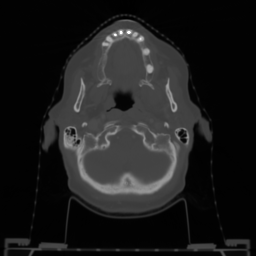
\includegraphics[width=\textwidth]{images/IMG0138_example.png}
      \caption{Original image}
    \end{subfigure}
    \hfill
    \begin{subfigure}[t]{.32\textwidth}
      \centering
      
\includegraphics[width=\textwidth]{images/IMG0138_MASS_example.png}
      \caption{Image mask}
    \end{subfigure}
    \hfill
    \begin{subfigure}[t]{.32\textwidth}
      \centering
      
\includegraphics[width=\textwidth]{images/IMG0138_merge_example.png}
      \caption{Mask applied to original}
    \end{subfigure}
  
    \caption[Images from the dataset]{
      Example of images from the dataset
    }
  \end{figure}
\end{frame}

\subsection{Neural Networks}
\begin{frame}{\insertsubsec}
  \begin{figure}
    \centering
    
\tikzset{
  pics/layer/.style n args = {3}{
    code = {
      \foreach \y in {1,...,#1} {
        \node[draw, circle] (L-#2-\y) at (0,{1.5*(\y - #1/2)}) {${#3}_{#2 \y}$};
      }
    }
  }
}

\begin{tikzpicture}
\def\layers{2/I, 5/H, 5/H, 3/O}

\foreach \x/\name [count=\xi] in \layers  {
  \draw (3*\xi, 0) pic {layer={\x}{\xi}{\name}};
}

\foreach \x/\ignore [count=\xi, remember=\xi as \lastxi, remember=\x as \lastx] in \layers {
  \ifthenelse{\xi > 1}{
    \foreach \ylast in {1,...,\lastx} \foreach \y in {1,...,\x}{
      \draw [-latex] (L-\lastxi-\ylast) -- (L-\xi-\y);
    }
  }{};
}

\end{tikzpicture}


    \caption[Neural network graph]{
      Neural Network graph drawing. 
    }
  \end{figure}
\end{frame}

\begin{frame}
  \begin{block}{Hidden Layers}
    \begin{equation*}
      \begin{aligned}
        z_i^{[l]} &= \sum_{j = 1}^{n^{[l]}} w_{ij}^{[l]} \cdot a_j^{[l - 1]} + w_{i0}^{[l]} \\
        a_i^{[l]} &= g^{[l]}(z_i^{[l]})
      \end{aligned}
      \quad
      \xrightarrow{\text{becomes}}
      \quad
      \begin{aligned}
        \bm{z}^{[l]} &= \bm{W}^{[l]} \cdot \bm{a}^{[l - 1]} + \bm{b}^{[l]} \\
        \bm{a}^{[l]} &= g^{[l]}(\bm{z}^{[l]})
      \end{aligned}
    \end{equation*}
  
  \end{block}
  \begin{figure}
    \centering
    
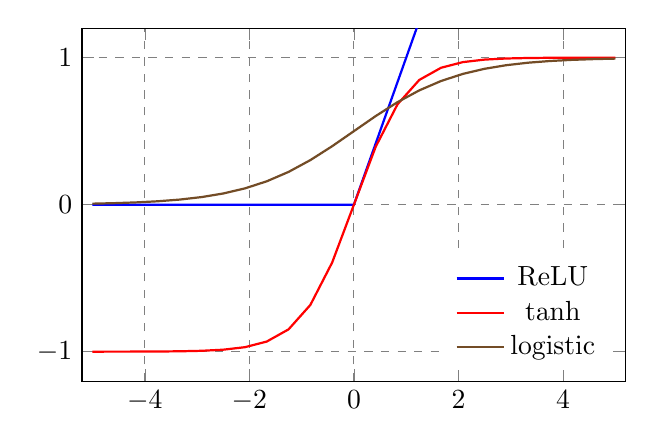
\begin{tikzpicture}
\begin{axis}[
    xmin = -5.2, xmax = 5.2,
    ymin = -1.2, ymax = 1.2,
    legend style = {draw = none},
    legend pos = south east,
    grid=major,
    grid style = {dashed, gray},
    width = 0.7\textwidth,
    height = 0.5\textwidth,
    every axis plot/.append style={thick},
    no markers,
    cycle list name = color
  ]
  \addplot{max(0, x)};
  \addplot{tanh(x)};
  \addplot{1/(1 + exp(-x))};
  \legend{ReLU, tanh, logistic}
\end{axis}
\end{tikzpicture}
  
    \caption[Activation functions]{
      Activation functions
    }
  \end{figure}
\end{frame}

\begin{frame}
  \begin{block}{Output layers}
    \[
      g_k^{[L]}(\bm{a}^{[L - 1]}) = \frac{e^{a_k^{[L - 1]}}}{\sum_{i = 1}^K e^{a_i^{[L - 1]}}}
    \]
  \end{block}
  
  \begin{block}{Cost function}
    \begin{align*}
      \hat{\bm{y}} &:= g^{[L]}(\bm{a^{[L - 1]}}) \\
      C(\bm{y}, \hat{\bm{y}}) &:= \frac{1}{N} \sum_{i = 1}^N (y_i - \hat{y}_i)^2
    \end{align*}
  \end{block}
\end{frame}

\subsection{Convolutional Neural Networks}

\begin{frame}{\insertsubsec}
  \centering
  \begin{figure}
    \hspace{-7cm}
    \adjustbox{max width=1.35\pagewidth}{\input{drawings/convolution_operation.tikz.tex}}

    \caption{Convolution operation}
  \end{figure}

  \begin{block}{Output size}
    \begin{align*}
      n_{\text{next}} = \left\lfloor\frac{n_{\text{prev}} + p - f}{s}\right\rfloor + 1
    \end{align*}
  \end{block} 
\end{frame}

\begin{frame}
  \begin{figure}
    \centering
    \scalebox{.7}{\input{drawings/convolutional_layer.tikz.tex}}
    \caption{Convolutional layer}
  \end{figure}

  \begin{align*}
    \bm{z}^{[l]} &= \bm{W}^{[l]} \cdot \bm{a}^{[l - 1]} + \bm{b}^{[l - 1]} \\
    &\downarrow \text{becomes} \\
    \bm{\mathsf{Z}}^{[l]} &= \bm{\mathsf{A}}^{[l - 1]} * \bm{\mathsf{W}}^{[l]} + 
    \bm{\mathsf{B}}^{[l - 1]}
  \end{align*}
\end{frame}
 
% !TEX root = ../main.tex

\section{Project scope}
\subsection{Problem formulation}
\begin{frame}{\insertsubsec}
  \begin{itemize}
    \item We have access to a unique set of \( \simeq 500 \) scans
    \item Develop a new deep learning model to analyze this dataset
    \item Get better results than the \emph{volume} radiomic feature which usually achieves
    a C-index of 0.65 for the Head and Neck dataset. 
  \end{itemize}
\end{frame}

\subsection{State-of-the-art}
\begin{frame}{\insertsubsec}
  The most typical approach is to extract radiomic features, usually with
  the \emph{PyRadiomics} package, from the MRI, PET or CT scans.

  \vspace{.5cm}
  An alternative approach is to use deep-learning based models for prediction or 
  feature extraction. Pre-trained models have reduced the requirements for big data sets.
  Possible strategies are:
  \begin{itemize}
    \item Use a pre-trained CNN as a feature extractor
    \item Fine tune a pre-trained CNN on medical data
  \end{itemize}
  
\end{frame}

\subsection{Stakeholders}
\begin{frame}{\insertsubsec}
  \begin{itemize}
    \item Developer: responsible for research, document and implement the software
    \item Director: responsible for guiding, giving advice and helping the Developer
    \item Beneficiaries: future researchers or patients depending on the outcome
  \end{itemize}
\end{frame}

\subsection{Methodology}
\begin{frame}{\insertsubsec}
  \begin{itemize}
    \item As a research project it will have a process of trial and error
    \item Once in a while the project will be presented in the lab weekly meetings
    \item Every week a meeting with the Principal Investigator will be scheduled
  \end{itemize}
\end{frame}

\subsection{Obstacles}
\begin{frame}{\insertsubsec}
  Some obstacles may be found during the project:

  \begin{itemize}
    \item Training time
    \item Bugs
    \item Scheduling
    \item Not enough data
  \end{itemize}
\end{frame}

% !TEX root = ../main.tex

\section{Design and implementation}

\subsection{Pre-process data}
\begin{frame}{\insertsubsec}
  \begin{itemize}
    \item Pre-process image data
    \item Pre-process scalar data
    \item Generate pairs for training
  \end{itemize}

  \vspace{.5cm}
  Only 490 of the initial 671 could be used to fit a model because we needed the following 
  requirements:
  \begin{itemize}
    \item CT scan
    \item Tumour annotations
    \item Radiomic features
    \item Clinical information
  \end{itemize}
\end{frame}

\begin{frame}{Image data pre-processing}
  \begin{figure}
    \centering
    \scalebox{.6}{\def\customimage{10em}
\begin{tikzpicture}[node distance = 2]
    \node (P-0) at (0, 0) {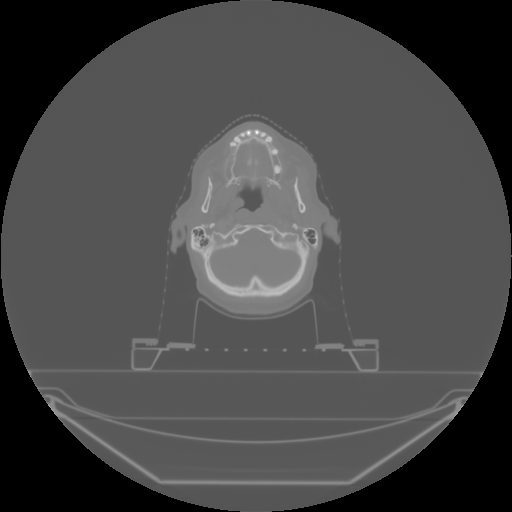
\includegraphics[width=\customimage]{images/preprocess/process_0}};
    \node [below = of P-0] (P-1) {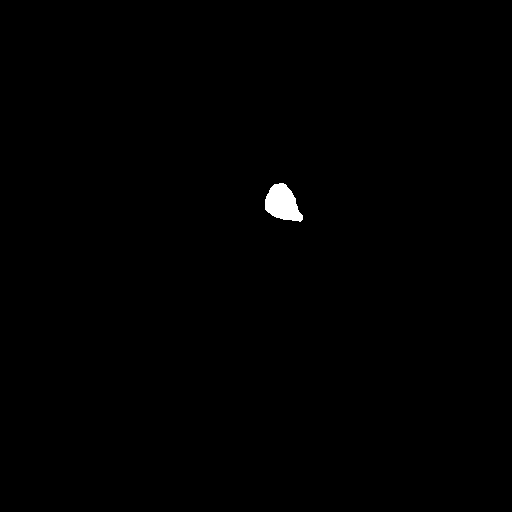
\includegraphics[width=\customimage]{images/preprocess/process_1}};

    \node [below = .2 of P-0] (text-0) {Scan};
    \node [below = .2 of P-1] (text-1) {Mask};
    
    \node [right = of P-1] (P-2-0) {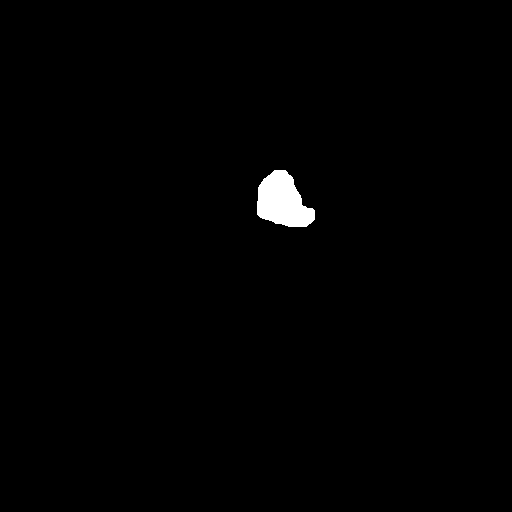
\includegraphics[width=\customimage]{images/preprocess/process_2_0}};
    \node [right = of P-2-0] (P-2-1) {
\includegraphics[width=\customimage]{images/preprocess/process_2_1}};
    \node [right = of P-2-1] (P-5) {
\includegraphics[width=\customimage]{images/preprocess/process_5}};
    
    \node [above = of P-2-1] (P-3) {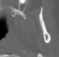
\includegraphics[width=\customimage]{images/preprocess/process_3}};
    \node [right = of P-3] (P-4) {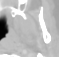
\includegraphics[width=\customimage]{images/preprocess/process_4}};

    \node [right = .5 of P-5, circle, draw] (prod) { \Large \( \times \) };
    
    \node [below = of P-5] (P-6) {
\includegraphics[width=\customimage]{images/preprocess/process_6}};
    \node [left = of P-6] (P-7) {
\includegraphics[width=\customimage]{images/preprocess/process_7}};
    \node [left = of P-7] (P-8) {
\includegraphics[width=\customimage]{images/preprocess/process_8}};

    \node [below = .2 of P-6] { \( 59 \times 57 \) px};
    \node [below = .2 of P-7] { \( 64 \times 64 \) px};
    \node [below = .2 of P-8] { \( 64 \times 64 \) px};

    \draw [-latex] (P-0) -- (P-3);
    \draw [-latex] (P-3) -- (P-4) node[midway, below, align=center] {Remove \\ extreme \\ values};
    \draw [-latex] (P-4) -| (prod);

    \draw [-latex] (P-1) -- (P-2-0) node[midway, below, align=center] {Gaussian \\ filter};
    \draw [-latex] (P-2-0) -- (P-2-1) node[midway, below, align=center] {Bounding \\ box};
    \draw [-latex] (P-2-1) -- (P-3) node[midway, right, align=center] {Slice};
    \draw [-latex] (P-2-1) -- (P-5) node[midway, below, align=center] {Slice};
    \draw [-latex] (P-5) -- (prod);

    \draw [-latex] (prod) |- (P-6) node[near end, below, align=center] {Apply \\ mask};
    \draw [-latex] (P-6) -- (P-7) node[midway, below, align=center] {
        Resize \\ \( 64 \times 64 \times 64 \)
    };

    \draw [-latex] (P-7) -- (P-8) node[midway, below, align=center] {Normalize};

\end{tikzpicture}}
    \caption{Image data pre-processing}
  \end{figure}
\end{frame}

\begin{frame}{Scalar data pre-processing}
  \begin{itemize}
    \item Clinical information
    \begin{itemize}
      \item Patient's ID
      \item Age
      \item Sex
      \item Survival event
      \item Survival time
    \end{itemize}
    \item Radiomic features, up to 725
    \begin{itemize}
      \item Tumour shape
      \item Intensity
      \item Volume
      \item ...
    \end{itemize}
  \end{itemize}
\end{frame}
\begin{frame}
  \begin{figure}
    \centering
    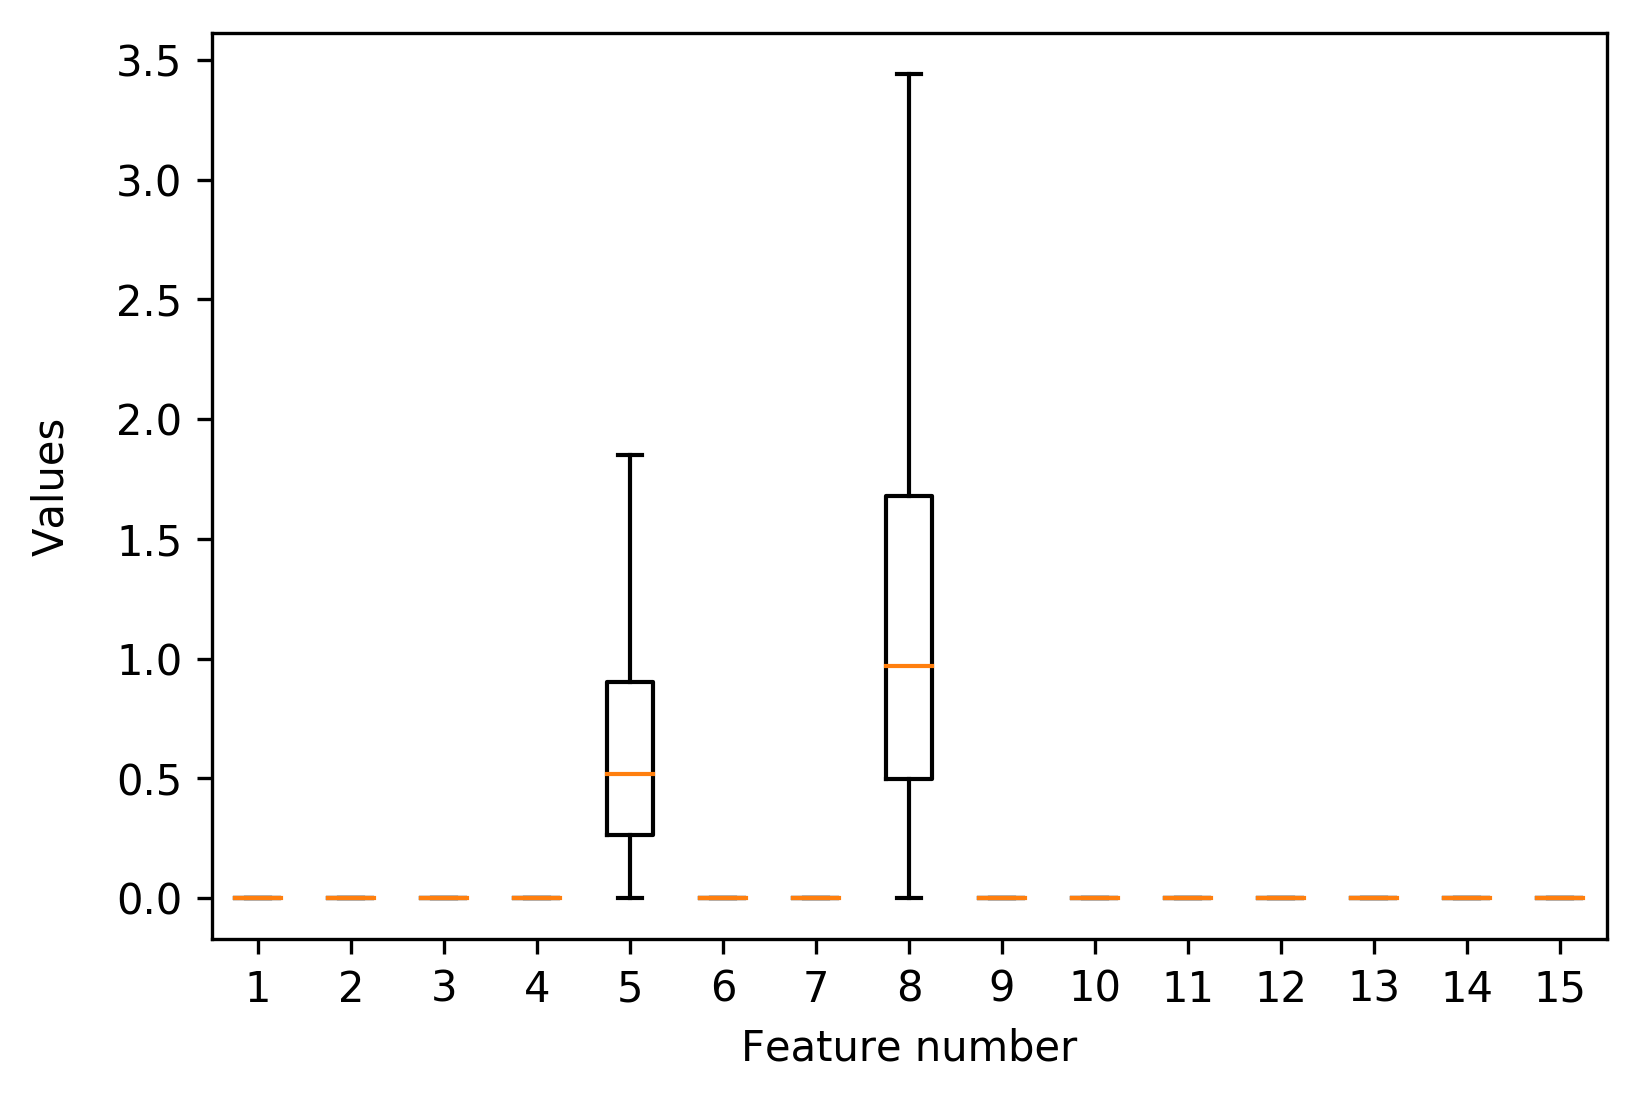
\includegraphics[width=\textwidth]{images/features_original}
    \caption{Features before normalization}
  \end{figure}
\end{frame}
\begin{frame}
  \begin{figure}
    \centering
    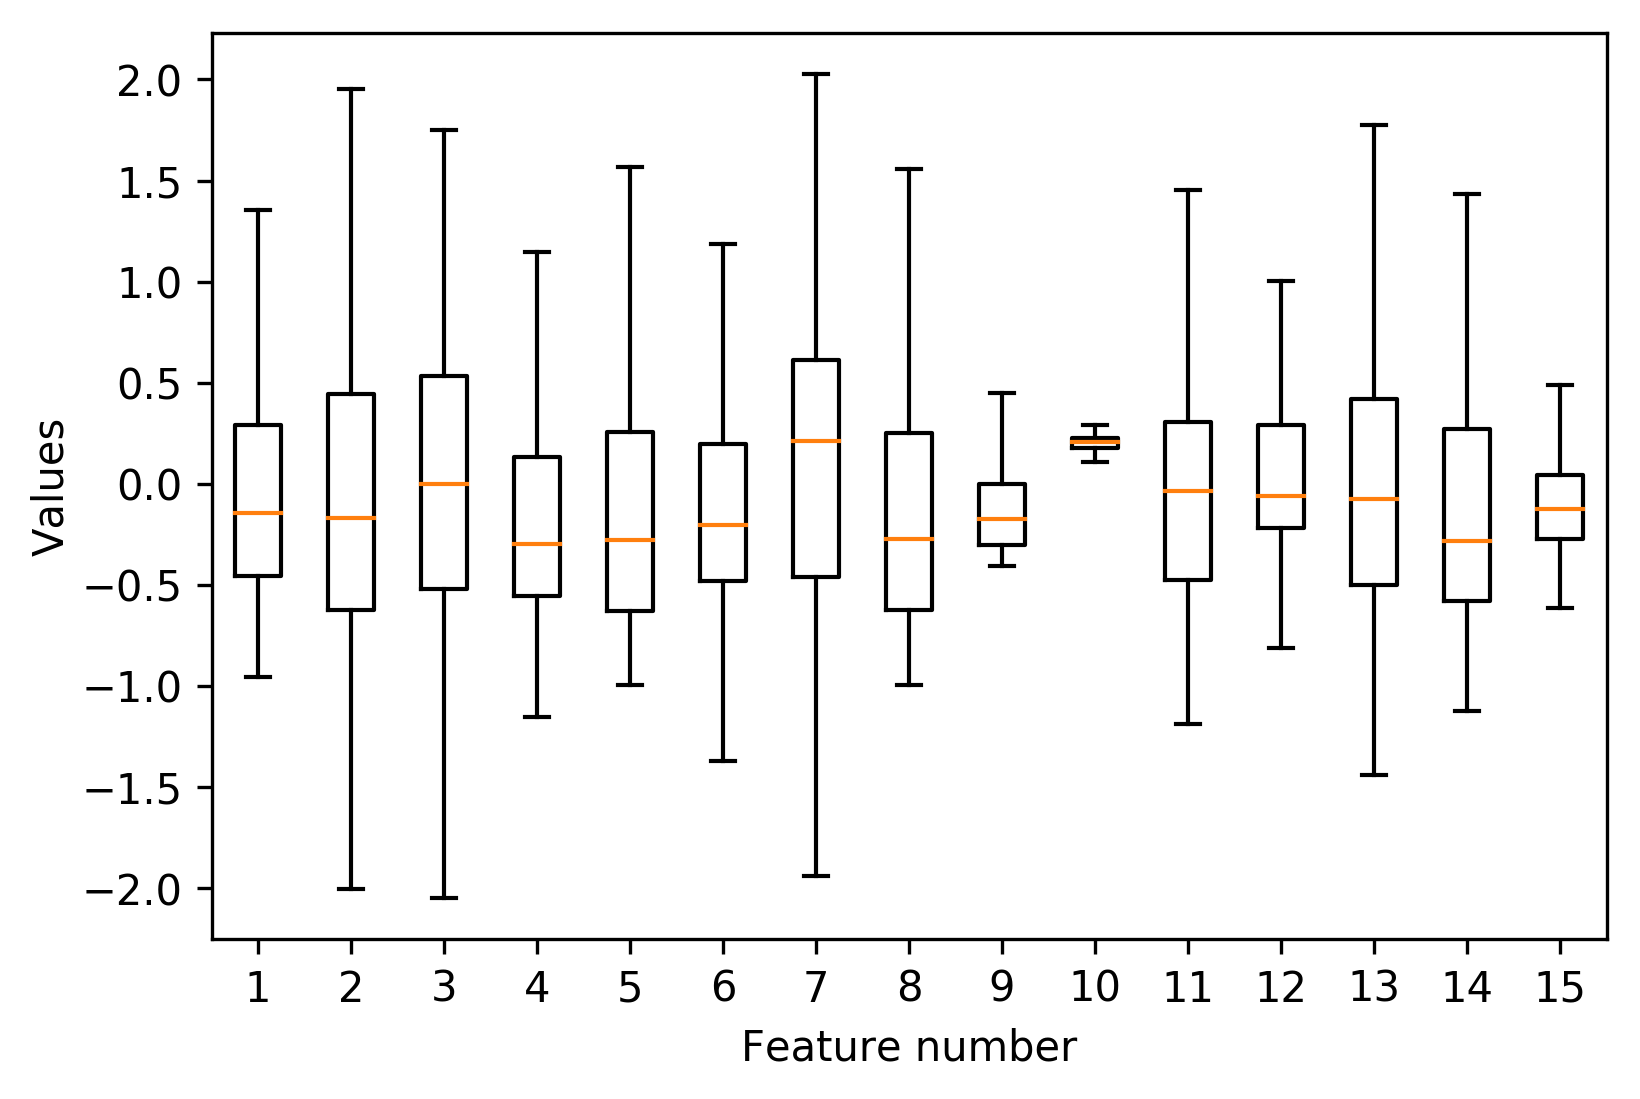
\includegraphics[width=\textwidth]{images/features_normalized}
    \caption{Features after normalization}
  \end{figure}
\end{frame}

\begin{frame}{Pair generation}
  
  \begin{figure}
    \centering
    \scalebox{.7}{\def\customimage{5em}
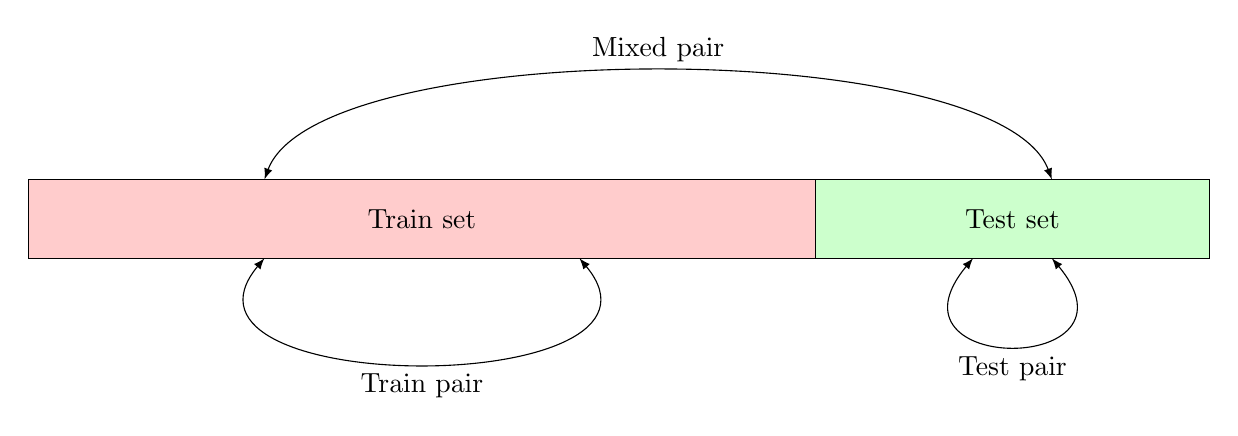
\begin{tikzpicture}
    
    \draw [fill = red!20] (0, 0) rectangle (10, 1);
    \draw [fill = green!20] (10, 0) rectangle (15, 1);

    \node at (5, .5) {Train set};
    \node at (12.5, .5) {Test set};

    \draw [bend right=130, latex-latex, looseness=1.5] (3, 0) to node [midway, below] {Train pair} (7, 0);
    \draw [bend right=130, latex-latex, looseness=5] (12, 0) to node [midway, below] {Test pair} (13, 0);
    \draw [bend left=70, latex-latex, looseness=.5] (3, 1) to node [midway, above] {Mixed pair} (13, 1);
\end{tikzpicture}}
    \caption{Types of pairs generated from train and test sets}
  \end{figure}

  \begin{block}{Conditions}
    \begin{itemize}
      \item Both of them are uncensored \( E_A = E_B = 1 \)
      \item The uncensored time of one is smaller than the censored time of the other
            \( T_A < T_B | E_A = 1; E_B = 0 \)
    \end{itemize}
  \end{block}
\end{frame}

\subsection{Create basic siamese model}
\begin{frame}{\insertsubsec}
  Step required from a software engineering perspective. Future models should implement the 
  \( \operatorname{sister}(x) \) function.

  \begin{align*}
    \bm{O}_A &= \operatorname{sister}(\bm{X}_A) \\
    \bm{O}_B &= \operatorname{sister}(\bm{X}_B) \\
    \sigma(x) &= \frac{1}{1 + \exp(-x)} \\
    \hat{y} &= \sigma(||\bm{O}_B||_2 - ||\bm{O}_A||_2) 
  \end{align*}

  \[
    \mathcal{L}(\bm{y}, \hat{\bm{y}}) = -\frac{1}{N} \sum_{i = 1}^{N}
    (1 - y_i)\log(1 - \hat{y}_i) + y_i\log(\hat{y}_i)
  \]

  \[
    C(\bm{y}, \hat{\bm{y}}) = \mathcal{L}(\bm{y}, \hat{\bm{y}}) + 
    ||\bm{w}||_2
  \]
\end{frame}

\subsection{Build volume only model}
\begin{frame}{\insertsubsec}
  Very simple model to have a baseline

  \[
    \operatorname{sister}(\bm{X}) = w\cdot X_{\text{scalar}_{26}} + b
  \]
\end{frame}
\begin{frame}
  Parameters:
  \begin{itemize}
    \item Learning rate: 0,05
    \item Number of epochs: 200
    \item Batch size: The whole dataset
  \end{itemize}

  Previous state-of-the-art CI was 0,628

  \begin{table}
    \centering
    \begin{tabular}{|c||c|c|c||c|c|c|}
      \cline{2-7}
      \multicolumn{1}{c|}{} & \multicolumn{3}{|c||}{\textbf{Pairs}} & 
      \multicolumn{3}{c|}{\textbf{Concordance Index}} \\
      \hline
      \textbf{Fold} & \textbf{Mixed} & \textbf{Train} & \textbf{Test} 
      & \textbf{Mixed} & \textbf{Train} & \textbf{Test} \\
      \hhline{=======}
      0 & 16.359 & 46.804 & 5.330 & 0,627 & 0,634 & 0,639 \\
      1 & 16.359 & 46.957 & 5.278 & 0,629 & 0,635 & 0,63 \\
      2 & 16.348 & 47.577 & 5.084 & 0,636 & 0,627 & 0,661 \\
      3 & 16.348 & 47.274 & 5.176 & 0,618 & 0,644 & 0,6 \\
      \hhline{=======}
      \textbf{Total} & 65.414 & 188.612 & 20.868 & 0,627 & 0,635 & 0,632 \\
      \hline
    \end{tabular}
  
    \caption[Volume Only 4-CV results]{
      Results for volume only model using 4-CV \label{tab:results-volume-4CV}
    }
  \end{table}
\end{frame}

\begin{frame}
  \begin{figure}
    \centering
    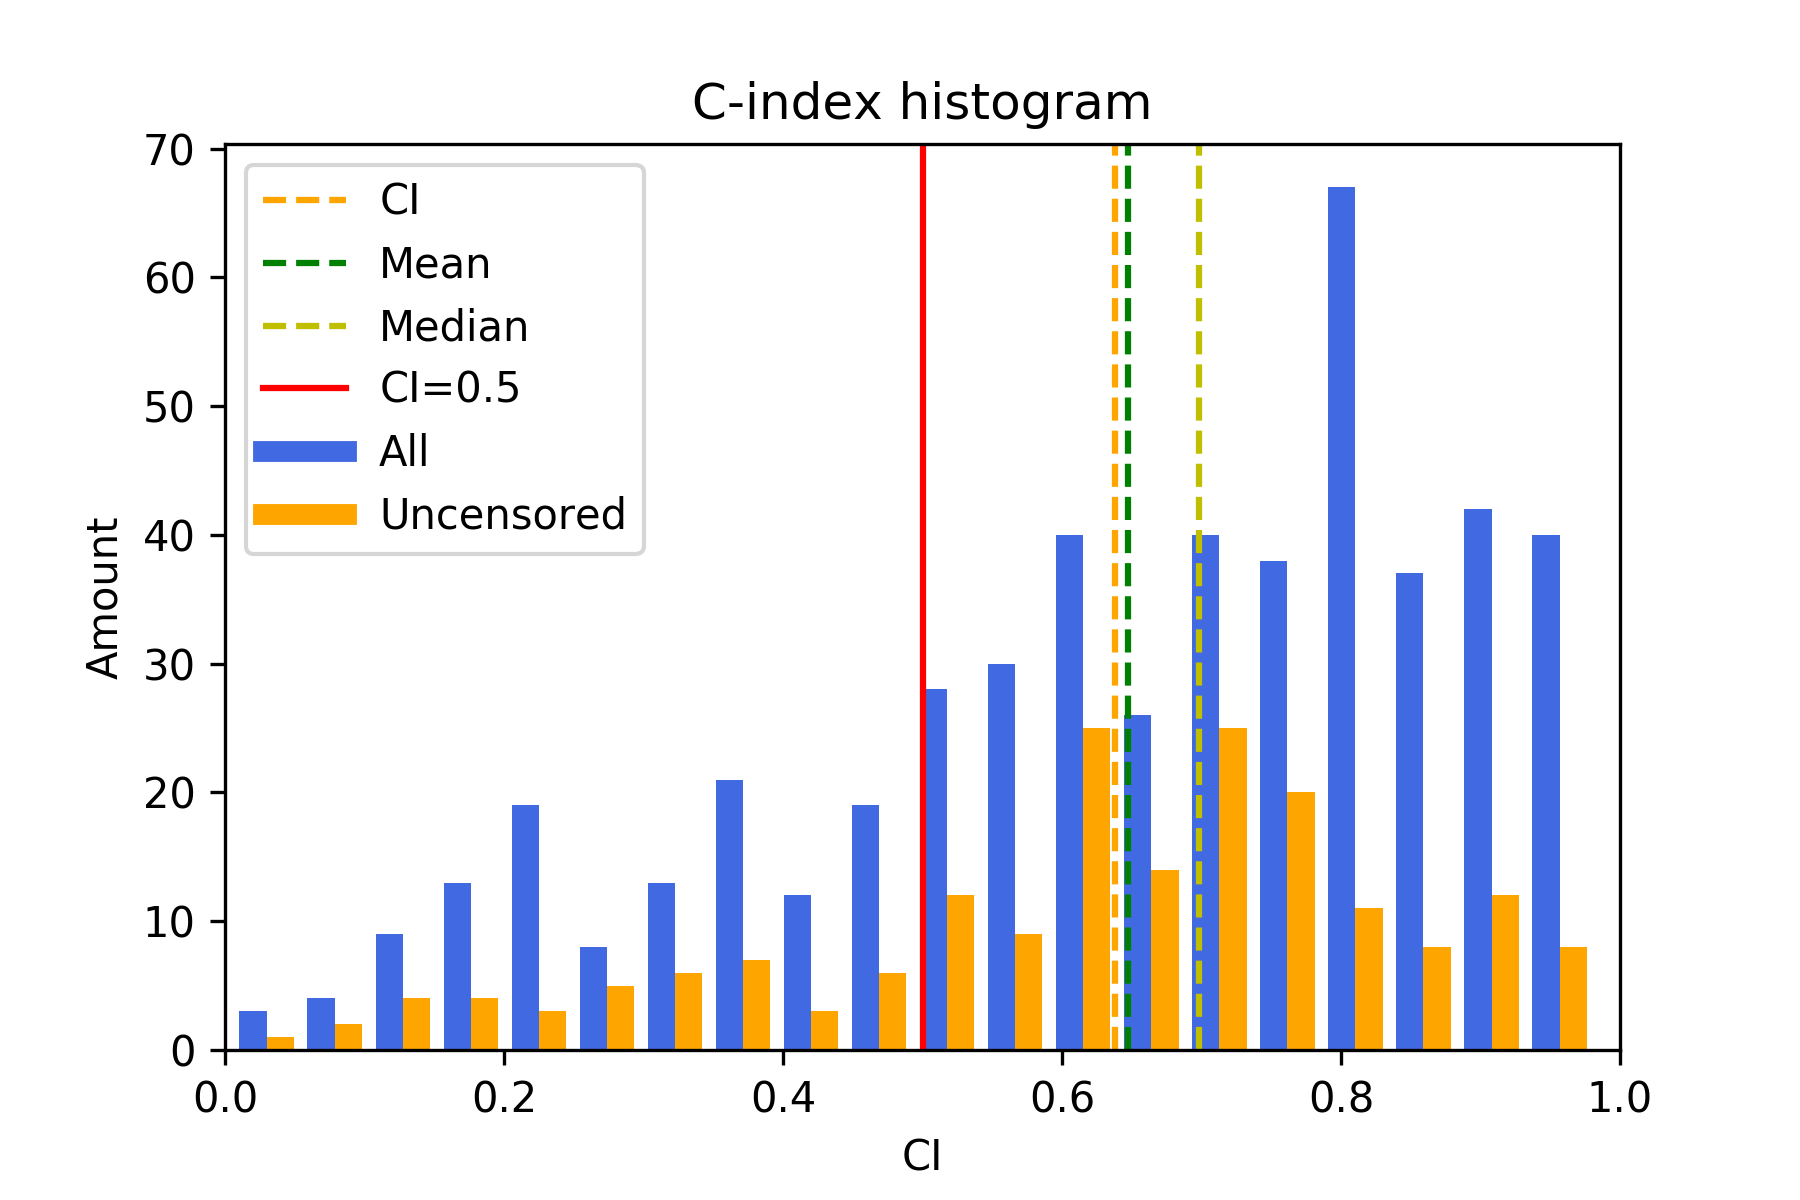
\includegraphics[width=.8\textwidth]{images/results/c-index_volume}
    \caption[LOOCV volume only model results]{
      Volume only model results using LOOCV \label{fig:results-volume-LOOCV}
    }
  \end{figure}
\end{frame}

\subsection{Build shallow siamese network}
\begin{frame}{\insertsubsec}
  \begin{figure}
    \centering
    \scalebox{.7}{
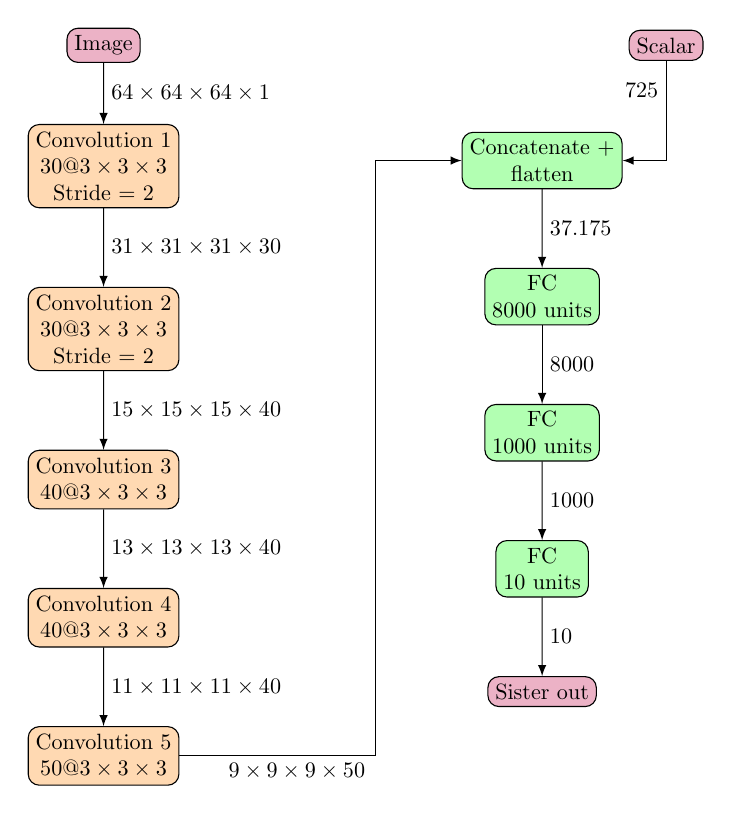
\begin{tikzpicture}[every node/.style={scale=.8}]

  \tikzstyle{module}=[rounded corners, draw, align=center]
  \tikzstyle{FC}=[module, fill=green!30]
  \tikzstyle{conv}=[module, fill=orange!30]
  \tikzstyle{io}=[module, fill=purple!30]
  
  
  \node [io] (image) {Image};
  \node [conv, below = of image] (CNN-1) at (0, 0) {
    Convolution 1 \\ 
    \( 30 @ 3 \times 3 \times 3 \) \\
    Stride = 2
  };
  \node [conv, below = of CNN-1] (CNN-2) {
    Convolution 2 \\
    \( 30 @ 3 \times 3 \times 3 \) \\
    Stride = 2
  };
  \node [conv, below = of CNN-2] (CNN-3) {
    Convolution 3 \\
    \( 40 @ 3 \times 3 \times 3 \)
  };
  \node [conv, below = of CNN-3] (CNN-4) {
    Convolution 4 \\
    \( 40 @ 3 \times 3 \times 3 \)
  };
  \node [conv, below = of CNN-4] (CNN-5) {
    Convolution 5 \\
    \( 50 @ 3 \times 3 \times 3 \)
  };

  \node [right = 5 of image] (aux) {};
  \node [io, right = of aux] (scalar) {Scalar};

  \node [FC, below = of aux] (con) {Concatenate + \\ flatten};
  \node [left = of con] (aux-2) {};
  \node [FC, below = of con] (FC-1) {FC \\ 8000 units};
  \node [FC, below = of FC-1] (FC-2) {FC \\ 1000 units};
  \node [FC, below = of FC-2] (FC-3) {FC \\ 10 units};

  \node [io, below = of FC-3] (out) {Sister out};
  
  \draw [-latex] (image) -- (CNN-1) node[midway, right] {\( 64 \times 64 \times 64 \times 1 \)};
  \draw [-latex] (CNN-1) -- (CNN-2) node[midway, right] {\( 31 \times 31 \times 31 \times 30 \)};
  \draw [-latex] (CNN-2) -- (CNN-3) node[midway, right] {\( 15 \times 15 \times 15 \times 40 \)};
  \draw [-latex] (CNN-3) -- (CNN-4) node[midway, right] {\( 13 \times 13 \times 13 \times 40 \)};
  \draw [-latex] (CNN-4) -- (CNN-5) node[midway, right] {\( 11 \times 11 \times 11 \times 40 \)};

  \draw (CNN-5) -| (aux-2.center)  node[pos=.3, below] {\( 9 \times 9 \times 9 \times 50 \)};
  \draw [-latex] (aux-2.center) |- (con);
  \draw [-latex] (scalar) |- (con) node[pos=.15, left] {\( 725 \)};
  
  \draw [-latex] (con) -- (FC-1) node[midway, right] {\( 37.175 \)};
  \draw [-latex] (FC-1) -- (FC-2) node[midway, right] {\( 8000 \)};
  \draw [-latex] (FC-2) -- (FC-3) node[midway, right] {\( 1000 \)};
  \draw [-latex] (FC-3) -- (out) node[midway, right] {\( 10 \)};
\end{tikzpicture}


}
    \caption{Shallow siamese sister's network illustration \label{fig:shallow-implement}}
  \end{figure}
\end{frame}



\section*{Acknowledgements}
\begin{frame}{Acknowledgements}
  \begin{itemize}
    \item Benjamin Haibe-Kains
    \item Maria Serna
  \end{itemize}
\end{frame}

\begin{frame}
    \begin{center}
        \LARGE Questions?
    \end{center}
\end{frame}

% !TEX root = ../main.tex

\begin{frame}{Technical competences}
  \begin{itemize}
    \item CCO1.1: Evaluate computational complexity. \emph{A little bit}
    \item CCO2.1: Demonstrate knowledge about the basics and paradigms of intelligent systems. 
    \emph{Enough}
    \item CCO2.4: Demonstrate knowledge and develop computational learning techniques. \emph{In depth}
    \item CCO2.5: Implement software for information retrieval. \emph{Enough}
  \end{itemize}
\end{frame}

\begin{frame}{Stem reduction}
  \begin{figure}
    \centering
    \scalebox{1.}{\input{drawings/residual_block_stem.tikz.tex}}
    \caption{Residual network Stem Block \label{fig:residual-block-stem}}
  \end{figure}
\end{frame}

\begin{frame}{Block A}
  \begin{figure}
    \centering
    \scalebox{.6}{\input{drawings/residual_block_a.tikz.tex}}
    \caption{Residual network convolutional Block A \label{fig:residual-block-a}}
  \end{figure}
\end{frame}

\begin{frame}{Reduction A}
  \begin{figure}
    \centering
    \scalebox{.85}{\input{drawings/residual_block_reduce_a.tikz.tex}}
    \caption{Residual network Reduction A \label{fig:residual-block-reduce-a}}
  \end{figure}
\end{frame}

\begin{frame}{Block B}
  \begin{figure}
    \centering
    \scalebox{.5}{\input{drawings/residual_block_b.tikz.tex}}
    \caption{Residual network Block B \label{fig:residual-block-b}}
  \end{figure}
\end{frame}

\begin{frame}{Reduction B}
  \begin{figure}
    \centering
    \scalebox{.9}{\input{drawings/residual_block_reduce_b.tikz.tex}}
    \caption{Residual network Reduction B \label{fig:residual-block-reduce-b}}
  \end{figure}
\end{frame}




\end{document}